%!TEX root = ../main.tex
% chktex-file 46
\chapter{Learning to Decompose Graphs}%
\label{sec:ltd}

In the last chapter we saw how existing \ac{gcr} approaches relate to \ac{lta}.
Despite their differences, all described \ac{lta} formulations have one thing in common:
Their decomposition functions $\psi$ all split a given graph $G$ into constituents spanned by \ac{bfs} subtrees of $G$ or simply into connected components of $G$.
The only exception to this is the \ac{lta} formulation of \acp{svm} that use fingerprint embeddings; there the constituents are all isomorphic to handpicked substructures.

Apart from the fingerprint embedding approach, which requires domain knowledge in order to pick meaningful substructure patterns, current \ac{gcr} approaches use constituents that are at-best \textit{localized} but not necessarily \textit{interpretable}.
The defining characteristic of \ac{lta} proposed in \cref{sec:ltag:definition}, \textit{localized explainability}, is therefore only partially satisfied by existing approaches.
This shortcoming of the existing \ac{lta} formulations for structured input data gives rise to a new problem:
\begin{defn}
	The \ac{ltd} problem is solved by finding a graph decomposition function $\psi: \mathcal{G}_{\mathcal{D}} \to \mathcal{P}(\mathcal{G}_{\mathcal{D}})$ which splits all graphs $G \in \mathcal{G}_{\mathcal{D}}$ from a given domain $\mathcal{D}$ into constituent subgraphs which are individually ``meaningful'' in the domain $\mathcal{D}$.
\end{defn}

As per our definition of \ac{lta} from \cref{sec:ltag:definition}, the quality of an \ac{lta} formulation is determined by its chosen solution for the \ac{ltd} problem.
Since a comprehensive analysis of this problem would be beyond the scope of this thesis, we focus on the relation between \ac{ltd} and \acp{gcnn}.
The goal of this chapter is to answer the following two questions:
\begin{enumerate}
	\item \textit{Can a stack of graph convolution layers learn a decomposition function dynamically instead of using a static subtree decomposition?}
	\item \textit{What could be the foundation for such an ``\acs{ltd}-convolution'' layer?}
\end{enumerate}

We provide an answer to the first question in \cref{sec:ltd:edge-filter} by showing how decomposition functions $\psi$ can be learned via so-called \textit{edge filters} as part of a convolutional \ac{gnn} architecture.
This establishes the connection between the \acs{ltd} problem and graph convolutions on a high level.
Then the second question is tackled in \cref{sec:ltd:kgnn-limits,sec:ltd:wl2gnn}.
There a novel graph convolution approach is proposed which could serve as a starting point for a convolution layer which solves the \ac{ltd} problem.

\section{Learning Constituents via Edge Filters}%
\label{sec:ltd:edge-filter}

As we saw in \cref{sec:ltag:formulation:gcnn:conv}, the constituents of neighborhood convolutions are spanned by \ac{bfs} trees of depth $T$, where $T$ is the number of convolutional layers.
From this perspective the problem of learning constituents corresponds to learning a pruning operator on the branches of \ac{bfs} trees.
Such a pruning operator filters the edges that are traversed in each \ac{bfs} step.
There are two general edge filtering strategies:
\begin{enumerate}[label={\textbf{\arabic*.}}]
	\item \textbf{Edge prefiltering:}
		Here the edge filtering and convolution operations are performed in independent steps:
		First the edges of a given graph are filtered, then the convolution layers are applied to the filtered graph.
		This so-called \textit{edge prefiltering} strategy is illustrated in \cref{fig:ltd:subtree-filtering}.
		The main advantage of prefiltering is that it allows arbitrary combinations of edge filtering and convolution approaches.
		The main disadvantage is however that the same edges are removed in all \ac{bfs} subtrees.
		This restricts the expressive power of the learned decomposition function as shown in \cref{fig:ltd:dynamic-subtree-filtering}.
	\item \textbf{Dynamic edge filtering:}
		By filtering edges as part of the convolution operation itself, more flexible decompositions can be obtained.
		In the \textit{dynamic edge filtering} strategy the edge filter is part of the convolution operation and decides which neighbors of a given root node should be aggregated.
		Using this strategy a decomposition such as that shown in \cref{fig:ltd:dynamic-subtree-filtering} is learnable.
\end{enumerate}
\begin{figure}[ht]
	\centering
	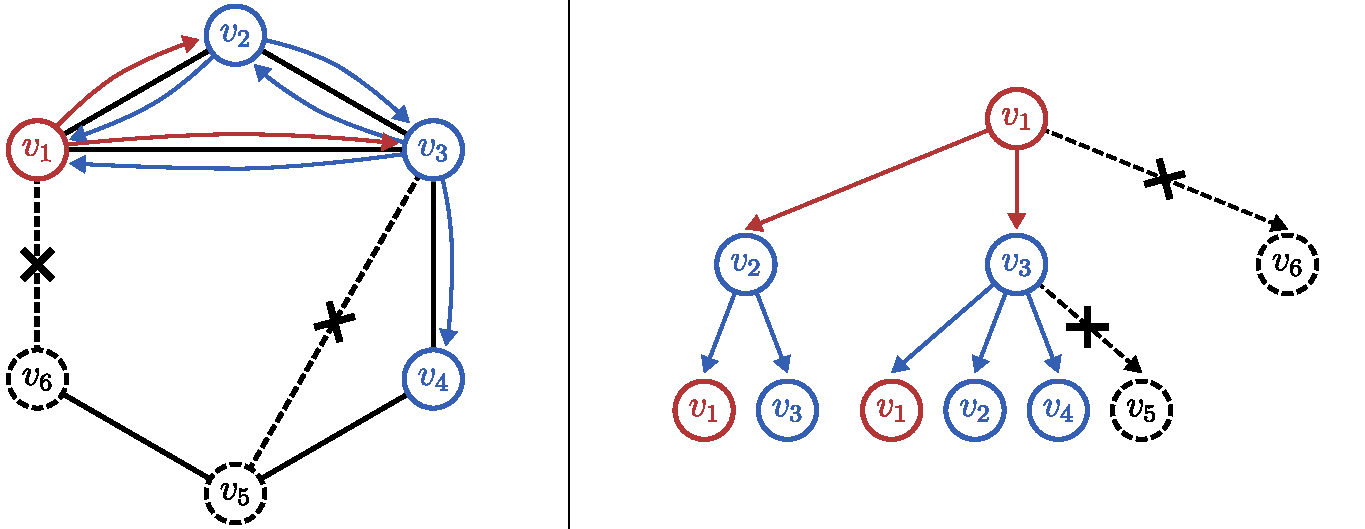
\includegraphics[width=0.8\linewidth]{gfx/ltd/subtree-filtering.pdf}
	\caption{Illustration of a pruned \ac{bfs} subtree when two edges are removed via prefiltering.}\label{fig:ltd:subtree-filtering}
\end{figure}
\begin{figure}[ht]
	\centering
	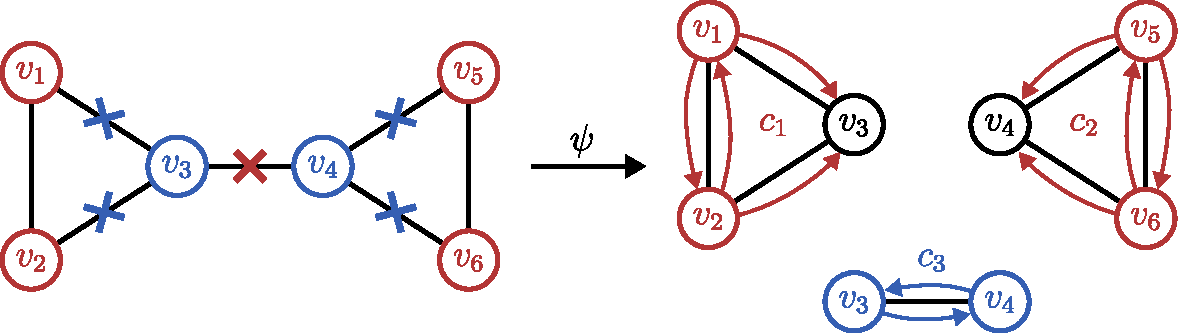
\includegraphics[width=0.75\linewidth]{gfx/ltd/dynamic-subtree-filtering.pdf}
	\caption[A graph decomposition obtained via dynamic edge filtering which cannot be modeled by edge prefiltering.]{
		A graph decomposition obtained via dynamic edge filtering which cannot be modeled by edge prefiltering.
		Depending on the \ac{bfs} root node $v_{\mathrm{root}}$ different edges are removed.
		For $v_{\mathrm{root}} \in \textcolor{t_blue}{\{ v_3, v_4 \}}$ the edges $\{ (v_3, v_1), (v_3, v_2), (v_4, v_5), (v_4, v_6) \}$ are filtered out while for $v_{\mathrm{root}} \in \textcolor{t_red}{\{ v_1, v_2, v_5, v_6 \}}$ the edge $(v_3, v_4)$ is removed. % chktex 25
	}\label{fig:ltd:dynamic-subtree-filtering}
\end{figure}
Irrespective of the chosen edge filtering strategy, the decision whether to remove a given edge $e_{ij} = (v_i, v_j)$ or not has to be made based on relevant information about $e_{ij}$ and its surroundings.
One way to encode the information about $e_{ij}$ is via an edge feature vector $z_{ij} \in \mathbb{R}^d$ that is fed into the edge filter.

We propose that those edge feature vectors can be obtained via a 2-\acs{wl} inspired graph convolution layer since 2-\acs{wl} colors naturally represent the structural roles of edges as described in \cref{sec:related:character:wl}.
We already saw a \ac{gcnn} architecture in \cref{sec:related:gcr:nn} which could potentially compute such 2-\acs{wl} inspired edge feature vectors, the $k$-\acs{gnn}~\cite{Morris2019}.
Its variant for $k = 2$ produces edge feature vectors that can be used as the input for an edge filter.
However, as we will see in the next section, there are significant limitations to the discriminative and computational power of 2-\acsp{gnn}.

\section{Limitations of the Existing 2-\acs*{gnn}}%
\label{sec:ltd:kgnn-limits}

The $k$-\acs{gnn} is a \ac{gcnn} inspired by the $k$-\ac{wl} algorithm, it convolves feature vectors of vertex $k$-multisets.
In this section we will compare its $k = 2$ variant with the 2-\ac{wl} algorithm.
The main difference between the two boils down to their notion of ``neighborhood''.
As already briefly mentioned in \cref{sec:related:gcr:nn}, 2-\acsp{gnn} define the neighbors of an edge $\textcolor{t_blue}{e_{ij}} = (v_i, v_j)$ to be the edges that are incident to either $v_i$ or $v_j$. % chktex 25
In 2-\acs{wl} on the other hand, the neighbors of $\textcolor{t_blue}{e_{ij}}$ are the edge pairs ${\left\{(\textcolor{t_red}{e_{il}}, \textcolor{t_darkgreen}{e_{lj}})\right\}}_{v_l \in \mathcal{V}_G}$, i.e.\ all possible paths of length two that start at $v_i$ and end at $v_j$. % chktex 21 chktex 25
This difference becomes clear when comparing the definition of convolution in 2-\acsp{gnn} with that of color refinement in 2-\acs{wl} (see \cfullref[ on ]{eq:related:kgnn-layer} and \cfullref[ on ]{defn:related:wlk-refine}):
\begin{alignat*}{4}
	\text{2-\acs{gnn}\footnotemark: } && Z^{(t)}[e_{ij}] &= \sigma\Biggl( \textcolor{t_blue}{Z^{(t-1)}[e_{ij}]} W^{(t)} + &&\left( \smashoperator[r]{\sum_{v_l \in \Gamma_G(v_j)}} \textcolor{t_red}{Z^{(t-1)}[e_{il}]} + \smashoperator[lr]{\sum_{v_l \in \Gamma_G(v_i)}} \textcolor{t_darkgreen}{Z^{(t-1)}[e_{lj}]} \right) W_{\Gamma}^{(t)} \Biggr) \\ % chktex 25
	\text{2-\acs{wl}: } && \chi_{G,2}^{(t)}(e_{ij}) &= h\Bigl(\textcolor{t_blue}{\chi_{G,2}^{(t-1)}(e_{ij})}, &&\ldblbrace (\textcolor{t_red}{\chi_{G,2}^{(t-1)}(e_{il})}, \textcolor{t_darkgreen}{\chi_{G,2}^{(t-1)}(e_{lj})})\, |\, v_l \in \mathcal{V}_G \rdblbrace\Bigr) % chktex 25
\end{alignat*}\footnotetext{
	To highlight the relation between 2-\acsp{gnn} and 2-\acs{wl}, a 2-\acs{gnn} definition that is not generally correct is shown here;
	for self-loops with $i = j$ it incorrectly sums the feature vectors of neighboring edges twice.
	The correct general formula uses a single sum over $v_l \in {\Gamma_G(v_j) \cup \Gamma_G(v_i)}$.
}\begin{figure}[ht]
	\centering
	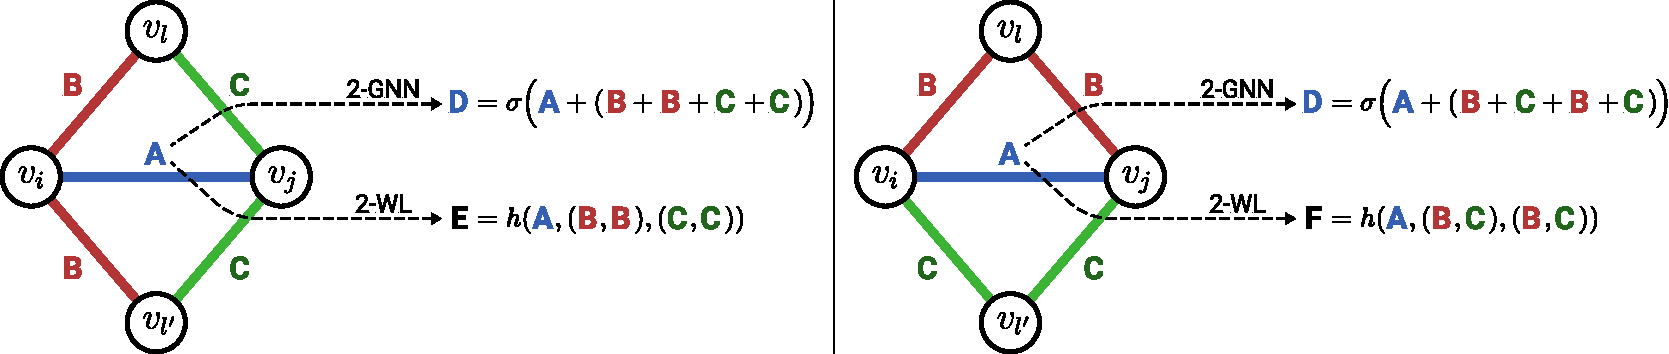
\includegraphics[width=\linewidth]{gfx/ltd/2gnn-2wl-diff.pdf}
	\caption[Edge colorings on which 2-\acsp{gnn} and 2-\acs{wl} behave differently.]{
		Two edge colorings on which 2-\acsp{gnn} and 2-\acs{wl} behave differently.
		A 2-\acs{gnn} will refine the ``color vector'' of $e_{ij}$ to \textsf{\textbf{\small\textcolor{t_blue}{D}}} for both initial colorings.
		2-\acs{wl} on the other hand differentiates both colorings by preserving the color tuple information.
	}\label{fig:ltd:2gnn-2wl-diff}
\end{figure}

We will now analyze what those different notions of neighborhood imply for the discriminative and computational power of 2-\acsp{gnn} in comparison to 2-\acs{wl}.
In the first step we show that the discriminative power of 2-\acsp{gnn} on all graphs $G \in \mathcal{G}$ is upper bounded by that of 1-\acs{wl} on the so-called \textit{edge neighborhood graphs} $G^{\mathcal{E}} \in \mathcal{G}^{\mathcal{E}}$.
\begin{defn}\label{defn:ltd:edge-graph}
	The \textit{edge neighborhood graph} of a given graph $G = (\mathcal{V}_G, \mathcal{E}_G)$ is defined as $G^{\mathcal{E}} \coloneqq (\mathcal{V}_{G^{\mathcal{E}}}, \mathcal{E}_{G^{\mathcal{E}}})$ with the vertices $\mathcal{V}_{G^{\mathcal{E}}} \coloneqq \{ \ldblbrace v, u \rdblbrace\, |\, (v, u) \in \mathcal{E}_G \lor v = u \}$ and the edges $\mathcal{E}_{G^{\mathcal{E}}} \coloneqq \left\{ (e, e') \in \mathcal{V}_{\mathcal{G}^{\mathcal{E}}}^2 |\, \left|e \cap e'\right| = 1 \right\}$. % chktex 21
\end{defn}
\begin{prop}\label{prop:ltd:2gnn-wl1-limit}
	The discriminative power of all 2-\acsp{gnn} $h_2$ is bounded by that of 1-\ac{wl} on edge neighborhood graphs, i.e.\ $\forall\, G, H \in \mathcal{G}: G^{\mathcal{E}} \mathrel{\simeq_1} H^{\mathcal{E}} \rightarrow h_2(G) = h_2(H)$. % chktex 21
\end{prop}
\begin{proof}
	By \cref{defn:ltd:edge-graph} it holds that $\forall e_{ij} \in \mathcal{E}_G: {\Gamma_G(v_i) \cup \Gamma_G(v_j)} = \Gamma_{G^{\mathcal{E}}}(e_{ij})$.
	Therefore the 2-\acs{gnn} convolution operation defined in \cfullref[ on ]{eq:related:kgnn-layer} can be rewritten as a vertex neighborhood convolution operator
	\begin{align*}
		Z^{(t)}[e] = \sigma\left( Z^{(t-1)}[e] W^{(t)} + \smashoperator[lr]{\sum_{e' \in \Gamma_{G^{\mathcal{E}}}(e)}} Z^{(t-1)}[e'] W_{\Gamma}^{(t)} \right)
		\text{.}
	\end{align*}
	\Cref{prop:ltd:2gnn-wl1-limit} then follows from \cref{prop:related:gcnn-wl1-limit}~(\cpageref{prop:related:gcnn-wl1-limit}).
\end{proof}
\begin{lem}\label{lem:wl1-regular-edge-neighbor-limit}
	1-\ac{wl} cannot distinguish the edge neighborhood graphs $G^{\mathcal{E}}$ and $H^{\mathcal{E}}$ of any pair of $d$-regular graphs $G$ and $H$ with $n$ vertices.
\end{lem}
\begin{proof}
	Let $G$ and $H$ be two $d$-regular graphs of size $n$.
	Their corresponding edge neighborhood graphs $G^{\mathcal{E}}$ and $H^{\mathcal{E}}$ both have $n^{\mathcal{E}} = n + \frac{nd}{2}$ vertices.
	$n$ of those edge neighborhood vertices correspond to the vertices of $G$ and $H$ respectively, we will refer to them as \textit{loop vertices} $L_G$/$L_H$.
	The remaining $\frac{nd}{2}$ edge neighborhood vertices correspond to the edges of $G$ and $H$, we will refer to them as \textit{edge vertices} $E_G$/$E_H$.

	W.l.o.g.\ we define the initial colors of the loop vertices as $\chi^{(0)}(v) = \textcolor{t_blue}{\texttt{A}}$ for all $v \in L_G \cup L_H$. % chktex 25
	The initial colors of the edge vertices are defined as $\chi^{(0)}(e) = \textcolor{t_red}{\texttt{B}}$ for all $e \in E_G \cup E_H$. % chktex 25
	Note that each loop vertex $\ldblbrace v_i, v_i \rdblbrace$ with $v_i \in \mathcal{V}_G \cup \mathcal{V}_H$ has $d$ neighbors, the edges incident to $v_i$.
	Similarly each edge vertex $\ldblbrace v_i, v_j \rdblbrace$ has $2d$ neighbors, two of which are the loop vertices $\ldblbrace v_i, v_i \rdblbrace$ and $\ldblbrace v_j, v_j \rdblbrace$ with the remaining $2d - 2$ neighbors corresponding to the edges that are incident to $e_{ij}$.

	After one color refinement step we then get $\chi^{(1)}(v) = h(\textcolor{t_blue}{\texttt{A}}, \ldblbrace \underbrace{\textcolor{t_red}{\texttt{B}}, \dots, \textcolor{t_red}{\texttt{B}}}_{d\text{ times}} \rdblbrace) \eqqcolon \textcolor{t_blue}{\texttt{C}}$ for all loop vertices $v \in  L_G \cup L_H$ and $\chi^{(1)}(e) = h(\textcolor{t_red}{\texttt{B}}, \ldblbrace \textcolor{t_blue}{\texttt{A}}, \textcolor{t_blue}{\texttt{A}}, \underbrace{\textcolor{t_red}{\texttt{B}}, \dots, \textcolor{t_red}{\texttt{B}}}_{\mathclap{2d - 2 \text{ times}}} \rdblbrace) \eqqcolon \textcolor{t_red}{\texttt{D}}$. % chktex 25
	This means that $\chi^{(0)}$ and $\chi^{(1)}$ are identical up to the color substitutions $\textcolor{t_blue}{\texttt{A}} \to \textcolor{t_blue}{\texttt{C}}$ and $\textcolor{t_red}{\texttt{B}} \to \textcolor{t_red}{\texttt{D}}$, i.e.\ $\chi^{(0)} \equiv \chi^{(1)}$, which in turn implies that 1-\ac{wl} terminates after one iteration. % chktex 25
	\Cref{lem:wl1-regular-edge-neighbor-limit} then directly follows since both $G^{\mathcal{E}}$ and $H^{\mathcal{E}}$ have $n$ vertices with the final color $\textcolor{t_blue}{\texttt{C}}$ and $\frac{nd}{2}$ vertices with the final color $\textcolor{t_red}{\texttt{D}}$, i.e.\ $G^{\mathcal{E}} \mathrel{\simeq_1} H^{\mathcal{E}}$. % chktex 25
\end{proof}
\begin{cor}
	A 2-\acs{gnn} cannot distinguish $d$-regular graphs and therefore has a lower discriminative power than 2-\ac{wl}.
\end{cor}
\begin{proof}
	The corollary directly follows from \cref{prop:ltd:2gnn-wl1-limit}, \cref{lem:wl1-regular-edge-neighbor-limit} and the fact that 2-\acs{wl} is able to distinguish most regular graphs~\cite[cor.~1.8.6]{Immerman1990}.
\end{proof}

\section{A Novel 2-\acs*{wl}-inspired \acs*{gnn}}%
\label{sec:ltd:wl2gnn}

\subsection{Definition of the 2-\acs*{wl} Convolution Operator}%
\label{sec:ltd:wl2gnn:definition}

\subsection{Expressive Power of 2-\acs*{wl}-\acsp*{gnn}}%
\label{sec:ltd:wl2gnn:properties}

\subsection{Implementation of 2-\acs*{wl}-\acsp*{gnn} on \acsp*{gpgpu}}%
\label{sec:ltd:wl2gnn:implementation}
